%% It is just an empty TeX file.
%% Write your code here.
\chapter{Experiment I}

Various signals transmitted in industrial environment have different requirements in terms of dependability. Let's consider a simple CCTV video transmission system. Each frame, even in low resolution solutions, consists of several hundred thousands pixels. The frame rate lies somewhere between 30 and 5 frames per second, depending on the requirements. Even multiple bit error in the compressed video information bitstream leads just to the corruption of some frames. Depending on the error rate and frame rate, such disturbance may not influence the correct service at all, just lowering the video quality. The system, despite some errors, still fulfills it's function. 
On the other hand the information flow between the control system and the nodes, placed on the robotic arms on the assembly line, consists in constant transmission of the coordinates of the destination and position of the arm. An error in such information can lead to the damage of manipulated objects or another catastrophic system failure.
Moreover, the quality of the signal propagation in such a rapidly changing environment is not constant. The error rate can significantly rise for a short time, but be relatively low otherwise. Spending time, power and resources on complex encoding and decoding may not be justified for the majority of the systems life time. The ability to adapt to the quality of the transmission would be just another advantage of well designed communication system.
In conclusion, the requirements of the industrial wireless system are diversified and need a configurable solution, that could offer a constantly high level of dependability while adapting to its environment and the use case. The high level of dependability means also the coverage of the non-recurrence of the Fault Tolerance. In other words, the channel encoders and decoders have to be reliable themselves.


\section{FEC in wireless communication}\label{sec:PENCA}
The theory behind the creation of Error Correction Codes (ECC) has been presented in \autoref{sub:codered}. The detection and correction of single bit errors can be achieved using a simple Hamming code \ref{art:Hamming}. With Hsaio Code or extended Hamming Code the single error correction and double error detection is possible \ref{book:Fujiwara,art:Hsiao}. Unfortunately in such a noisy and harsh environment as industrial production site, there may be faults causing more than one or two bit flips in the data bitstream. For such purposes the multiple-bit correcting codes like Reed-Solomon code \ref{Redd-Solomon} or BCH Code \ref{BCH} are suggested. They typically require much more effort in  encoding and especially in decoding the information. They tend to be slower. There are also other methods to deal with correction of two-bit errors like \ref{Hosp, Varghese}. All these proposals lack a simple one-fits-all solution, that could be used and configured to the needs of the target system and it's environment.

\begin{figure}[h]
\centering
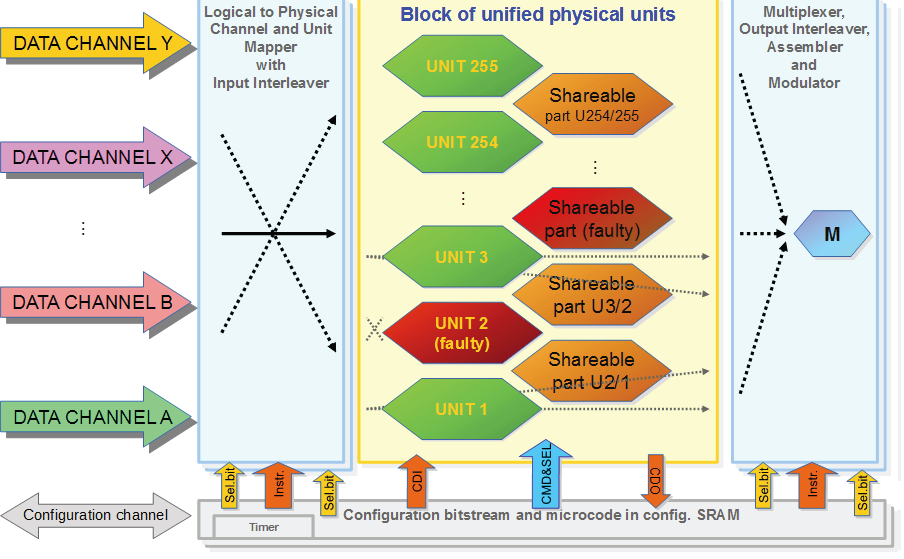
\includegraphics[width=0.25\textwidth]{figures/PENCA.png}
\caption{Basic scheme of the new dependable PENCA architecture~\cite{art:Pfeifer}}
\label{fig:PENCA}
\end{figure}

Programmable Encoder Architecture (PENCA) designed by P. Pfeifer and H. T. Vierhaus, firstly introduced in \ref{art:Pfeifer}, showed in~\autoref{fig:PENCA}, is an answer to the strict requirements of the dependable communication systems. The core of the solution consists in the "honeycomb" structure of units. The units can be replaced by neighboring units in case of errors detected in one of them. The internal test can be performed automatically or on demand. After testing, the unit can be marked as faulty, once the test fails, and its functionality logically remapped into another unit. Both the input and output units are implemented in two copies, since they are single points of failure and in case of permanent fault detected wouldn't be able to get repaired without a spare. The control of the system is done through the microcode (secured with parity bits). But above all, the architecture can be configured to serve as different channel encoders, starting with the implementation of the single error correcting codes and ending with the multiple-bit error correcting codes or even cross-parity codes. It is done via generation of polynomials by each unit and sometimes even borrowing resources from neighboring units for more extended polynomial generations. Each unit being able to perform BCH generator polynomial length task up to 42 coefficients (34 BCH codes) or 65 coefficients (50 BCH codes) with borrowed resources.
\subsection{Test of PENCA core}
The Unit Under Test is the internal core of the PENCA. The version is simplified and is not driven by opcodes, but by the 64-bit configuration bit-stream that sets all units to their desired functionality. The goal of the test is functional validation of the system and detection of its maximum frequency. For this purpose a Test Bench described in~\autoref{sec:Test_Bench} was used.
The components of Petr Pfeifer's composition, have been delivered as VHDL source file. The interface of the design is shown in \autoref{fig:PENCA_interface}.

\begin{figure}[h]
\centering
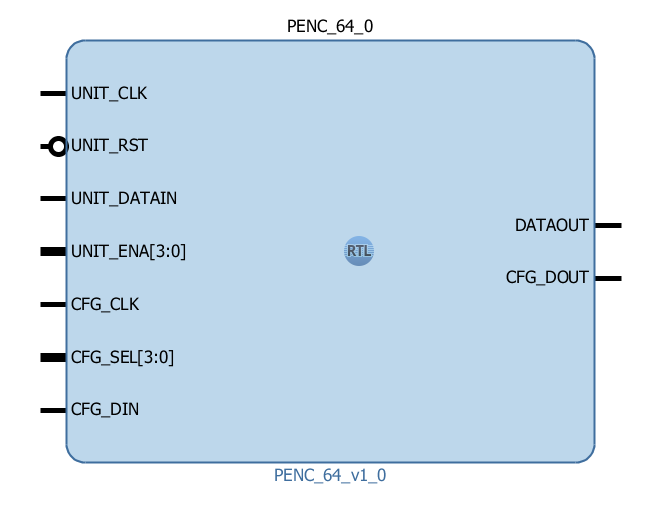
\includegraphics[width=0.25\textwidth]{figures/PENCA_interface.PNG}
\caption{Interface of PENCA}
\label{fig:PENCA_interface}
\end{figure}

To test the design in hardware it needs to be translated from the behavioral description into a real FPGA structure. The first stage of processing the design, after writing the source code, is the elaboration which translates the VHDL source code into electronic structures, like registers, logic gates, etc. This allows the designer to see if his concept, written as text, is describing the hardware properly.
The elaboration of the design and study on the source code reveals a repetitive structure of the design. The logic of the first two modules is shown in \autoref{fig:unit}. There are two clocks in the design. One clock is responsible for shifting in the configuration bit-stream, the other clock tacts the internal units, data input and output. Yellow elements are registers, that separate the successive sequential states from each other. They are the only sequential parts of the design. The clouds represent combinational logic, where outputs are logical functions of the inputs. This representation of the logic helps to keep the schematic clear and readable. the only important information are the inputs and outputs of the clouds. The trapezoid stays for multiplexer, forwarding one of the inputs to the output. Multiplexers are also parts of the combinational logic, since they are not driven by any clock and their output is a simple function of their inputs, but the schamatic profits when distinguishing then from the rest of the logic. The figure focuses on the data flow in the design, leaving the clocks aside. However one cannot forget that during each clock cycle, signals are propagated along the arrows and have to reach the registers inputs before the end of the cycle.

\begin{figure}[h]
\centering
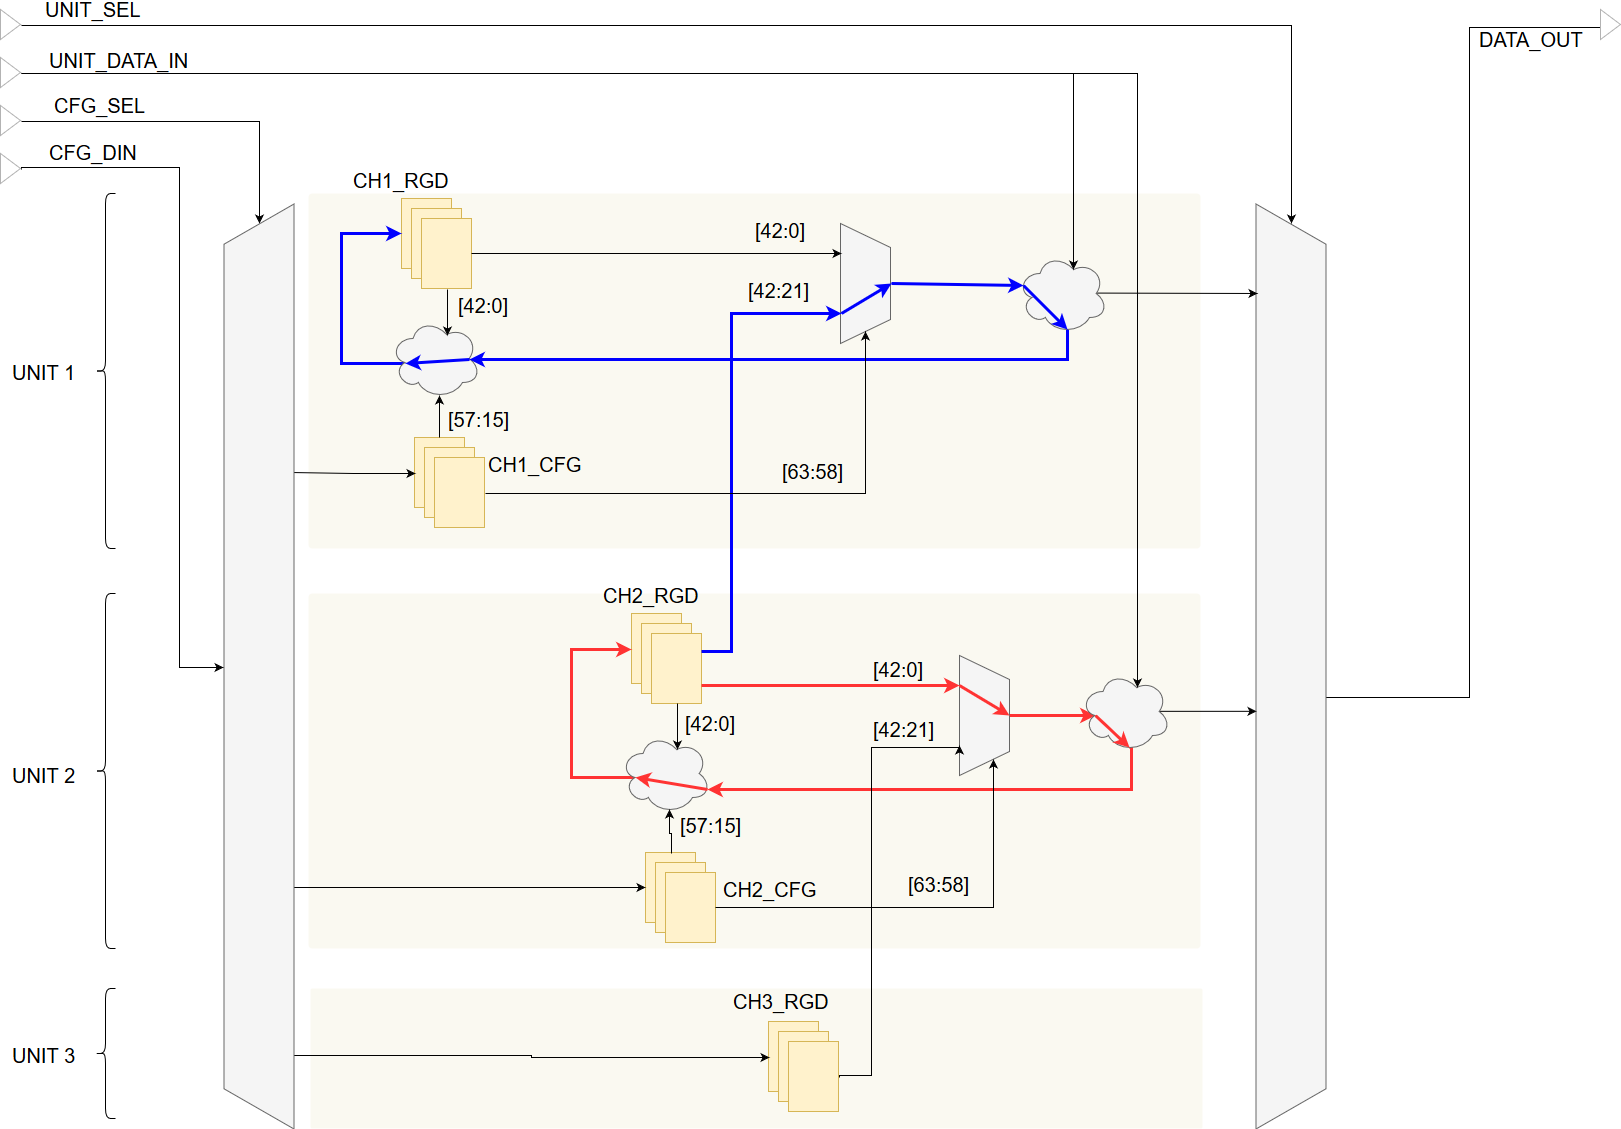
\includegraphics[width=\textwidth]{figures/Unit_arch.png}
\caption{Schematic of two PENCA units}
\label{fig:unit}
\end{figure}

\subsection{Structure Analysis}
Let us start with the configuration path, clocked with \textit{CFG\_CLK}. The configuration register is a shift register. Every Unit has its own configuration register and it can be chosen thanks to the simple addressing of \textit{CFG\_SEL}. After the analysis of the source code and the elaborated design, it is clear what the particular parts of the configuration bit-stream stand for. As visible in the \autoref{fig:unit}, the \textit{CHx\_CFG [57:15]} are parameters of the equation used in calculation of the parity bits for each unit. Each calculation step is stored back into \textit{CHx\_RGD} register. The \textit{CHx\_CFG [63:58]} selects which \textit{CHx\_RGD [i]} register is used for building a new parity bit and which \textit{CHx\_RGD} register will be used to calculate new value of the \textit{CHx\_RGD[i]} register. The \textit{CHx\_CFG [9:0]} is a counter value that indicates when to stop forwarding \textit{DATA\_IN} straight to the \textit{DATA\_OUT} and start building parity bits using \textit{CHx\_RGD[i]} register. The combinational logic used to calculate a new value of the \textit{CHx\_RGD[i]} register takes following inputs: the parameters stored in \textit{CHx\_CFG [57:15]}, the actual value of the \textit{CHx\_RGD[i-1]} and modified value of any other \textit{CHx\_RGD} or even \textit{CH(x+1)\_RGD}. The \textit{CH(x+1)\_RGD} stands for coefficients used in the next unit and only a half of those coefficients can be used in the calculation. The same applies for any unit, that uses all it's own coefficients and half of the coefficients of its successor.
\subsection{Design elaboration}
The elaboration process is actually a part of the project synthesis. It is creating a netlist that can be used by the synthesis tool to apply constraints to the design. It also maps the logic into FPGA internally used structures like Look Up Tables or Block Rams, but it doesn't decide where to place them yet. The mapping and netlist allow to conduct the first timing analysis, where the logic delays are known and the transportation delays are estimated. The Vivado IDE requires timing constraints to run the timing analysis. After the analysis, the tool reports back which paths did not fulfill the constraints. The speed of the design is determined by its longest/slowest path. The tool doesn't know yet the exact net delays but the estimation is usually helpful and lets the designer correct the source code before the design is placed in the actual target FPGA structure. In the case of the PENCA design there are two candidates for the longest possible path even before the synthesis. They are both marked in the \autoref{fig:unit}. The red path is the local feedback in calculation of the \textit{CHx\_RGD} and it is taken, when all coefficients used come from one unit. The blue path shows the situation when the coefficients are "borrowed" from the neighboring unit.
\subsection{Design Synthesis}
The synthesis tool shows that the path leading from the \textit{CH12\_RGD} to \textit{CH11\_RGD} is probably the longest path in the design and is estimated to take $5,061 ns$. The value is a sum of the logic delay $1,690 ns$ and the net delay $3,371 ns$. The path is shown in \autoref{fig:path}.

\begin{figure}[h]
\centering
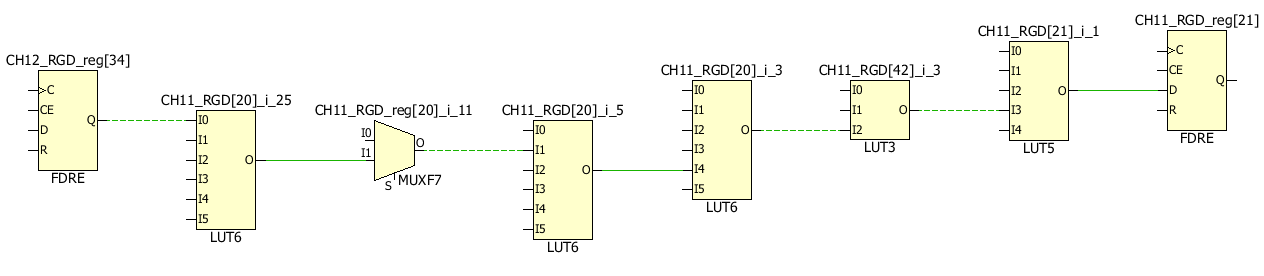
\includegraphics[width=\textwidth]{figures/path.png}
\caption{Longest synthesized path in the PENCA design}
\label{fig:path}
\end{figure}

The net delay is a double of the logic delay, which is caused by the fact, that the source register belongs to the 12th unit and the sink register to the 11th unit. The path corresponds to the blue scenario in \autoref{fig:unit}. The result of the synthesis is therefore a maximal possible frequency of the design, which theoretically comes to $197.589 MHz$. The high number of LUTs in the path is a result not only of the simple logical functions, but mostly because of the very big multiplexer, having 65 inputs. The multiplexing task is split into a simple multiplexer and row of LUTs.

\subsection{Design Implementation}
The last step of the work flow with the design is its implementation into the target architecture. The Look Up Tables and Memories and multiplexers are mapped into real CLBs of the target FPGA. The timing analysis in this step is the most accurate, that can be provided by the manufacturer. The only way to see the real cut-off frequency of the design is while testing it after the implementation. The UUT has to be placed in the FPGA with the Test Bench together in order to conduct the post-implemetation test. The result of the timing analysis 

\chapter{Experiment II}

The ParSec communication system (shown in~\autoref{fig:ParSec}) consists of:
\begin{itemize}
    \item MAC Layer processing, taking place within a standard processor, implemented mostly as software routines, interfaced with standard industrial bus.
    \item Forward Error Correction, as specialized reconfigurable hardware module
    \item followed by frame formatter
    \item Baseband processor, which consists of hardware processing and Radio Frequency units
\end{itemize}
The dependability of such a system is threatened by random errors in noisy channel, soft errors due to transient faults and hard errors due to permanent faults in hardware modules. Every ECC has its limits resulting from minimum hamming distance of its code space. The limits are oriented on the number of faults in one block and not on average fault rate of transmission channel. The following experiment aims at detecting the real correcting capabilities of ECC.
\section{Test of transmission path with known average error rate}
The Unit Under Test consists of one chosen, hard coded BCH(1023,948) encoder capable of correcting up to 8 bits per block. The decoder is followed by simple XOR gate, which overlays encoder output with error vector, simulating random errors in transmission path and transient errors in data processing digital logic laying on-path. The last module is the corresponding BCH decoder, with output indicating if the next data bit has been repaired or not. All modules are separated by flip-flops to simulate the delay that happens on the way between encoder and decoder. The error vector is supplied as just another input of the Test Bench.\\

The test starts with issuing the reset signal for one clock cycle, that will be propagated firstly to the encoder and later to the decoder input. The primary data input consists of $t$ randomly generated test vectors of length 948, followed by zeros to tact out the system response. The error vector has to be generated with care, to assure the exact average weight of all vectors and induce errors only within the block length. All error vectors are generated as one long vector with first $f_c$ bits set to one and rest to zero. The length of the vector is equal to $t\dot n$, where $n=1023$ is the length of a packet. The error vector is randomly permuted and split into $n$ vectors. The error vectors are shifted into the system along with input data, resulting in controlled corruption of encoder output. The erroneous data arrives at the decoder inputs just after the reset and gets processed 89 tacts before valid data appears on the data output. 

Prior to the test, few simulations were conducted, in order to see how many packets contain more errors $f_c$ than the code is able to correct. The test was suppose to validate, if the hardware module gives the same statistic of failed tests and therefore failed packets by known average error rate. The result is shown in~\autoref{fig:experiment2}.



\section{Functional Shorts Concept}
All modules of the communication system come in pairs that are complementary to each other. The demodulators task is to recreate the possible codeword \textbf{v} from the waveform received from the RF module. The same codeword that the modulator has translated into waveform in the transmitter. The waveform arriving at the receiver should match with the one sent by the transmitter (in ideal noiseless system). The channel decoder takes the code word and recreates the information sequence \textbf{u\^}, which previously entered the channel encoder. The signals, although maybe altered by transmission error or hardware error, should have the same form. The interface of each corresponding module of the receiver is an exact copy of the one placed in the transmitter, only exactly in the opposite direction. This ability can be used later for test purposes, excluding some modules from the communication path and feeding the corresponding modules with their pairs output directly.
If there was a possibility to exclude the noisy channel from the communication path, then all detected errors would have to have they origin within the hardware modules, indicating the presence of permanent faults. Such test could happed periodically or during the systems start up.
To implement such solution the transmitter would have to be directly connected with the receiver. Since communication modules are usually designed for both: transmitting and receiving, and all of their components come in complementary pairs, it would be possible to connect the outputs of transmitter modules to corresponding inputs of receivers modules. The idea of such "functional shorts" is shown in \autoref{fig:shorts}.
\subsection{System Partitioning for Test}
Another aspect of dependable communication systems is the wireless connection itself and the modulation used to provide the maximal insensitivity to multi-path propagation problems, fading effects and frequency interferences. The state-of-the art solutions incorporate Orthogonal Frequency Domain Multiplexing (OFDM) \ref{OFDM}, spread-spectrum communication \ref{spread-spectrum} or ultra wide-band frequency communication \ref{ultra wide-band}...
PSSS, 
 As mentioned in \autoref{ch:test} the testability of mixed signal and analog components is limited at best or requires instrumentation. 
